\section{Лучший за последнее время}

В разделе <<Лучшие за последнее время>> был выбран домен foxbox.pw. 

\begin{figure}[H]
    \centering
    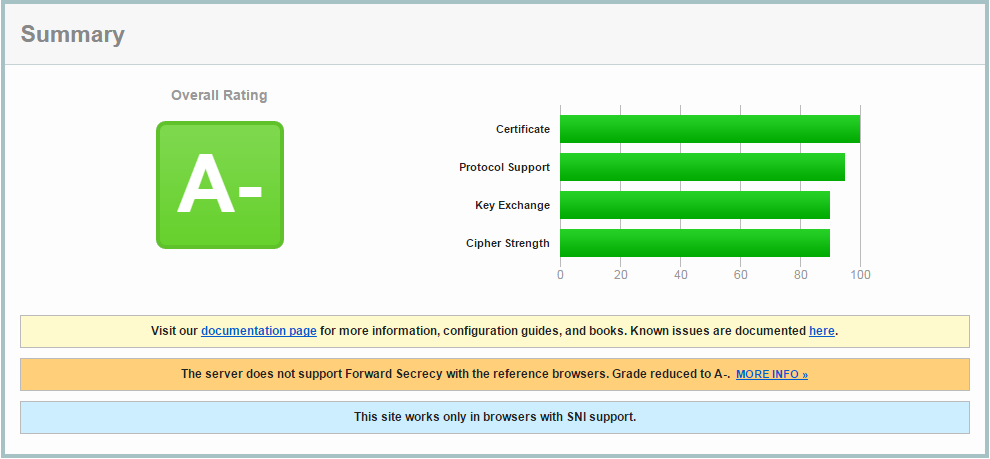
\includegraphics[width=\textwidth]{resources/01_summary.png}
    \caption{Сводка по домену foxbox.pw}
    \label{fig:01-summary}
\end{figure}

Оценка домена была снижена с \code{A} до \code{A-} поскольку продолжительная защищенность поддерживается не со всеми эталонными 
клиентами (браузерами).

Ниже приведена таблица рассшифровок шифров, доступных для использования на рассматриваемом домене. Колонки таблицы зашифрованы 
согласно нотации, представленной в разделе \ref{ssct:best-practices.configuration}.

\begin{table}[H]
    \centering
    \begin{tabular}{c|c|c|c|c|c}
        \textbf{P} & \textbf{KEA} & \textbf{AA} & \textbf{MEA} & \textbf{Мощность} & \textbf{HA} \\ 
        \hline
        TLS & RSA & RSA & 3DES\_EDE\_CBC & $168$ & SHA \\
        TLS & ECDHE & RSA & 3DES\_EDE\_CBC & $168$ & SHA \\
        TLS & RSA & RSA & AES\_128\_CBC & $128$ & SHA \\
        TLS & RSA & RSA & CAMELLIA\_128\_CBC & $128$ & SHA \\
        TLS & ECDHE & RSA & AES\_128\_CBC & $128$ & SHA \\
        TLS & RSA & RSA & AES\_128\_CBC & $128$ & SHA256 \\
        TLS & RSA & RSA & AES\_128\_GCM & $128$ & SHA256 \\
        TLS & ECDHE & RSA & AES\_128\_CBC & $128$ & SHA256 \\
        TLS & ECDHE & RSA & AES\_128\_GCM & $128$ & SHA256 \\
        TLS & RSA & RSA & AES\_256\_CBC & $256$ & SHA \\
        TLS & RSA & RSA & CAMELLIA\_256\_CBC & $256$ & SHA \\
        TLS & ECDHE & RSA & AES\_256\_CBC & $256$ & SHA \\
        TLS & RSA & RSA & AES\_256\_CBC & $256$ & SHA256 \\
        TLS & RSA & RSA & AES\_256\_GCM & $256$ & SHA256 \\
        TLS & RSA & RSA & AES\_256\_GCM & $256$ & SHA384 \\
        TLS & ECDHE & RSA & AES\_256\_CBC & $256$ & SHA384 \\
        TLS & ECDHE & RSA & AES\_256\_GCM & $256$ & SHA384 \\
    \end{tabular}
    \caption{Шифры, доступные на foxbox.pw}
    \label{tbl:01-cipher-suits}
\end{table}

Приведем теперь разбор некоторых деталий реализации протокола на рассматриваемом домене по категориям, рассмотренным в секции 
\ref{ssct:best-practices.protocol-details}

\begin{table}[H]
    \centering
    \begin{tabular}{c|c}
        \hline
        \multicolumn{2}{c}{\textbf{Уязвимости}} \\ \hline
        \textbf{Уязвимость} & \textbf{Уязвим} \\ \hline
        \textbf{DROWN} & Нет \\
        \textbf{BEAST} & Да, со стороны сервера \\
        \textbf{POODLE} & Нет \\
        \textbf{Атака на понижение версии} & Нет \\
        \textbf{Heartbleed} & Нет \\
        \textbf{OpenSSL CCS} & Нет \\
        \textbf{OpenSSL Padding Oracle} & Нет \\ \hline
        \multicolumn{2}{c}{\textbf{Опции}} \\ \hline
        \textbf{Опция} & \textbf{Включена} \\ \hline 
        \textbf{Безопасное переподключение} & Да \\ 
        \textbf{Сжатие данных} & Нет \\ 
        \textbf{Пульс} & Да \\ 
        \textbf{Продожительная защищенность} & Нет \\ 
        \textbf{ALPN} & Нет \\ 
        \textbf{NPN} & Да (HTTP/1.1) \\ 
        \textbf{Возобновление сессии (кэширование)} & Нет \\
        \textbf{Возобновление сессии (билеты)} & Да  \\
        \textbf{OCSP сшивание} & Да  \\
        \textbf{HSTS} & Нет \\ 
        \textbf{HPKP} & Нет \\ 
        \textbf{Отказ в длинном рукопожатии} & Нет \\ 
        \textbf{Отказ от версии} & Нет \\ 
    \end{tabular}
    \caption{Детали реализации протокола на foxbox.pw}
    \label{01-protocol-details}
\end{table}

Рассматриваемый домен поддерживает только протокол TLS, что уже свидетельствует о его не самой плохой защищенности. Кроме того, 
как видно из таблицы \ref{tbl:01-cipher-suits}, рассматриваемый домен не поддерживает RSA в качестве шифра для сообщений, что также
является большим плюсом. К тому же домен не подвержен ни одной известной SSL Server Test уязвимости (BEAST не считается --- полностью
клиентская уязвимость, как показано в разделе \ref{sssct:BEAST}). Единственным недостатком является частично не поддерживаемая 
продолжительная защищенность. 